%FOR PDFLATEX USE ONLY
\documentclass[a4paper,12pt]{article}

\usepackage{amssymb,amsmath} %math symbols

\usepackage[margin=2cm]{geometry} %paper geometry

\usepackage[utf8]{inputenc} %allows unicode (including russian) source file
\usepackage[russian]{babel} %docment in russian-style
\usepackage[utf8]{inputenc}
\usepackage[unicode]{hyperref} %links inside of the text
\usepackage[pdftex]{graphicx} %includegraphics pictures
\usepackage{cmlgc} %bold text

\usepackage{array} %arrays

\usepackage{wrapfig}
\usepackage{array}
\usepackage{lipsum}
\usepackage{esvect}
\usepackage{hyperref}
\usepackage{xcolor}
\definecolor{linkcolor}{HTML}{799B03} % цвет ссылок
\definecolor{urlcolor}{HTML}{799B03} % цвет гиперссылок
 
\hypersetup{pdfstartview=FitH,  linkcolor=linkcolor,urlcolor=urlcolor, colorlinks=true}
 
\usepackage{subfig}
\usepackage{calc}
\usepackage{pgfplots,tikz,circuitikz}
\usepackage{pgfplotstable}
\usepackage{tkz-euclide}

\usepackage{centernot}
\usepackage{cancel}

\documentclass{article}
\usepackage{amsmath}
\usepackage{mathtext}
\usepackage[T1,T2a]{fontenc}
\usepackage[utf8]{inputenc}
\usepackage[english, bulgarian, russian]{babel}
\usepackage{tikz}
\usepackage{pgfplots}
\usepackage[export]{adjustbox}
\usepackage[left=2cm,right=2cm,
    top=2cm,bottom=2cm,bindingoffset=0cm]{geometry}

\usepackage{csvsimple}

%\usepackage{centernot}
%\usepackage{cancel}

\begin{document}

\begin{center}
  \LARGE{Работа 1.2.1 LOL}\\[0.2cm]
  \LARGE{Определение скорости полета пули при помощи баллистического маятника}\\[0.2cm]
  \large{Боярина Екатерина,Воробьев Игорь}\\[0.2cm]
\end{center}

\textbf{Цель работы:} определить скорость полета пули, применяя законы сохранения и используя баллистические маятники.

\textbf{В работе используются:} духовое ружье на штативе, осветитель, оптическая система для измерения отклонений маятника, измерительная линейка, пули и весы для их взвешивания, а также баллистические маятники.

\section{Метод баллистического маятника, совершающего поступательное движение}
$L = (2.271\pm0.01)$ м - длина подвеса, $M=(2.925\pm0.005)$ кг - масса маятника.\\
Массы пуль (погрешность измерения 0.001 г):
\begin{figure}[h]
\begin{center}$
\begin{array}{|c|c|c|c|c|c|c|c|c|}
\hline
Номер & 1 & 2 & 3 & 4 & 5 & 6 & 7 & 8  \\
\hline
m\text{, г} & 0.514 & 0.508 & 0.506 & 0.494 & 0.502 & 0.496 & 0.499 & 0.502  \\
\hline
\end{array}$
\end{center}
\end{figure}

\begin{figure}[h]
\begin{center}$
\begin{array}{cc}
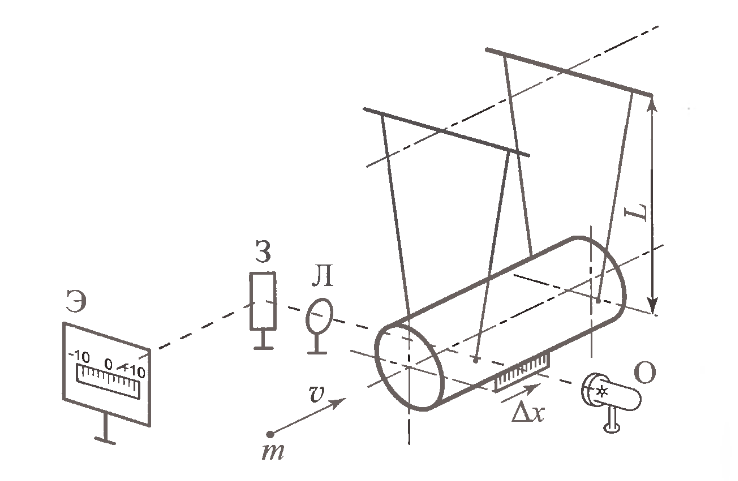
\includegraphics[width=0.45\textwidth]{picture_1.png}&
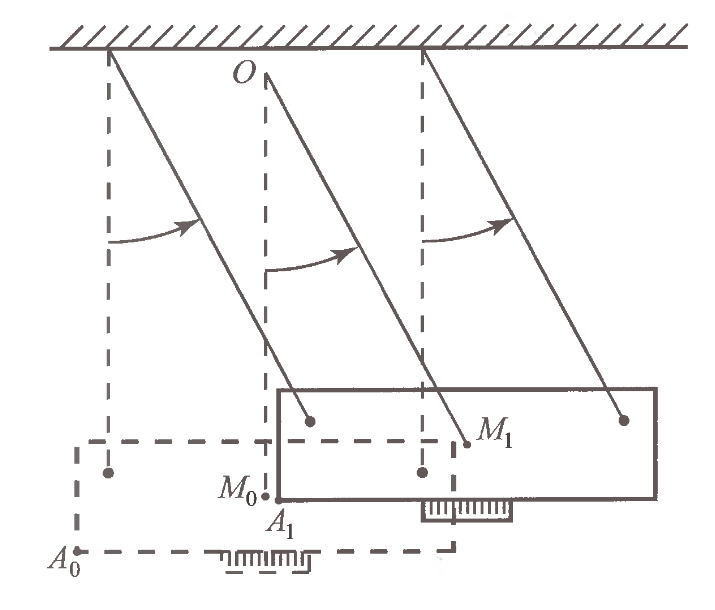
\includegraphics[width=0.45\textwidth]{picture_2.png}\\
\text{рис. 1. При попадании пули.} & \text{рис. 2. Перераспределение импульса.}\\
\end{array}$
\end{center}
\end{figure}

Распишем ЗСИ($u$ - скорость пули, $V$ - скорость маятника в нижней точке):
\begin{equation}
mu = V(M + m)
\end{equation}
Формула угловой скорости маятника $\omega = \sqrt{g/L}$. Формула скорости маятника в нижней точке через $A$(амплитуду) $V = A \omega$.
Выразим u:
\begin{equation}
u = \sqrt{\frac{g}{L}}\frac{M+m}{m}A
\end{equation}
\newpage

Таблица с результатами (погрешность $\Delta A$ = 0.5 мм):

\begin{figure}[h]
\begin{center}$
\begin{array}{|c|c|c|c|c|}
\hline
A\text{, мм} & 9.75 & 9.5 & 9.0 & 10.25\\
\hline
u\text{, м/c} & 116 & 114 & 108 & 127\\
\hline
\end{array}$
\end{center}
\end{figure}

Возьмем среднее $<u>=(116\pm4)\text{, м/c}$.

\section{Метод крутильного баллистического маятника}
\begin{figure}[h]
\begin{center}$
\begin{array}{c}
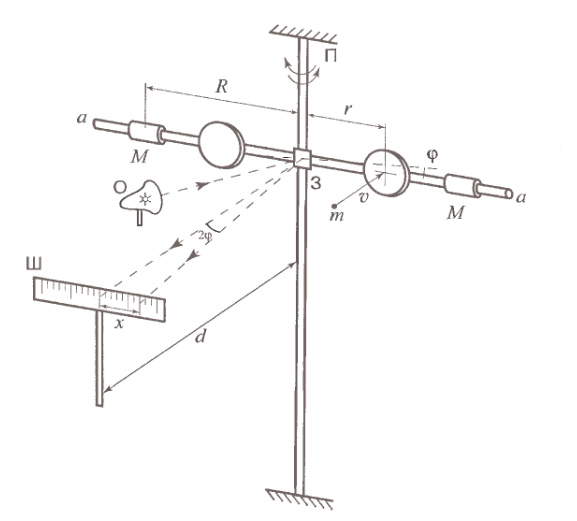
\includegraphics[width=0.73\textwidth]{picture_3.png}\\
\text{рис. 3. Установка.}
\end{array}$
\end{center}
\end{figure}

После попадания пули в мишень маятника, маятника начнет двигаться с $\omega$ (угловой скоростью). ЗСИ ($I$ -- момент инерции):
\begin{equation}
m v r = I \omega
\end{equation}
ЗСЭ ($k$ - модуль кручения проволоки, $\varphi$ - амплитуда):
\begin{equation}
k \frac{\varphi^2}{2} = I \frac{\omega^2}{2}
\end{equation}
Выразим $u$:
\begin{equation}
v = \varphi \frac{\sqrt{kI}}{mr}
\end{equation}
Выразим $\varphi$ из геометрии установки:
\begin{equation}
\varphi = \frac{|atan(\frac{x_0}{d})|}{2}
\end{equation}

Теоретически посчитаем $T_1$ и $T_2$:
\begin{equation*}
T_1 = 2 \pi \sqrt{\frac{I}{k}}
\end{equation*}
\begin{equation*}
T_2 = 2 \pi \sqrt{\frac{I - 2 M R^2}{k}}
\end{equation*}

Выразим из формул $\sqrt{k I}$:
\begin{equation*}
\sqrt{\textit{kI}} = \frac{4 \pi M R^2 T_1}{T_2^2 - T_1^2}
\end{equation*}

Измерим экспериментально: $T_1 = 13.77 с$, $T_2 = 17.99 с$

Таблица с результатами (погрешность $\Delta x$ = 5 мм):
\begin{figure}[h]
\begin{center}$
\begin{array}{|c|c|c|}
\hline
x, мм & $\varphi$, рад & u, м/с\\
\hline
105 & 0.142 & 122\\
\hline
100 & 0.136 & 118\\
\hline
95 & 0.129 & 112\\
\hline
100 & 0.135 & 116\\
\hline
\end{array}$
\end{center}
\end{figure}

Возьмем среднее $<u> = (117 \pm 2)\text{м/c}$.

\section{Вывод}
Ответы, сделанные разными методами, сходятся - это означает что вероятнее всего все было посчитано верно, а значит оба способа подходят для измерения момента инерции пули.
\end{document}








\lipsum[1-4]
\begin{wrapfigure}{R}{5cm}
\centering
\includegraphics[width=0.20\textwidth]{rd.png}
\caption{1}
\end{wrapfigure}
\lipsum[1-6]


\begin{figure}[h]
\begin{center}$
\begin{array}{cccc}
\includegraphics[width=0.20\textwidth]{rd.png}&
\includegraphics[width=0.20\textwidth]{rd.png}&
\includegraphics[width=0.20\textwidth]{rd.png}&
\includegraphics[width=0.20\textwidth]{rd.png}\\
(1) & (2) & (3) & (4)
\end{array}$
\end{center}
\end{figure}
